\documentclass{beamer}

\usepackage{graphicx}
\graphicspath{{./}}

\title{Quantitative Forecasting}

\begin{document}

\frame {
	"Forecasting is the process of making predictions of the future based
	on past and present data and most commonly by analysis of trends. A
	commonplace example might be estimation of some variable of interest at
	some specified future date."\\*
	– Wikipedia (https://en.wikipedia.org/wiki/Forecasting)
}

\frame {
	Why forecasting?
}

\frame {
	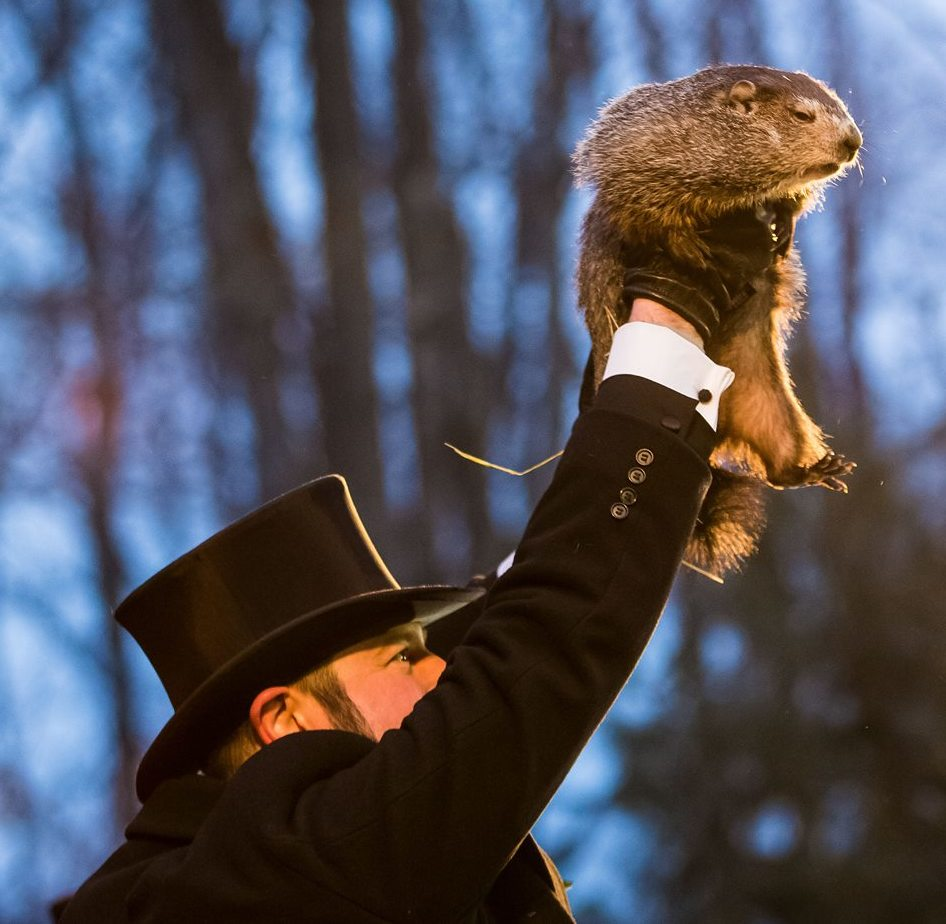
\includegraphics[width=\textwidth, height=\textheight, keepaspectratio=true]{groundhog}
}

\frame {
	Many things effective altruism is interested in take place in the future:
	\begin{itemize}
	\item Results of studies
	\item New technologies (clean meat, artificial intelligence, genetic engineering)
	\item Global risks (from biotechnology, artificial intelligence)
	\end{itemize}
}

\frame {
	Knowing about the extent \& frequency of these events is useful
}

\frame {
	Why quantitative?
}

\frame {
	\begin{itemize}
	\item Big difference between 1\% and 0.00001\% (especially with existenial risks!)
	\item Can be useful in expected value calculations
	\item This is effective altruism
	\end{itemize}
}

\frame {
	Central concepts
}

\frame {
	Probabilistic beliefs
}

\frame {
	It is possible \& useful to assign probabilities to some beliefs,
	as opposed to believing that X definitely will/won't happen.
}

\frame {
	Calibration
}

\frame {
	Example:
	\begin{itemize}
	\item I make 10 forecasts about the occurrence of radioactive rain in the next days
	\item For each day, I assign 60\% probability to "There will be radioactive rain"
	\item I'm calibrated if there is radioactive rain on 6 of these days
	\end{itemize}
}

\frame {
	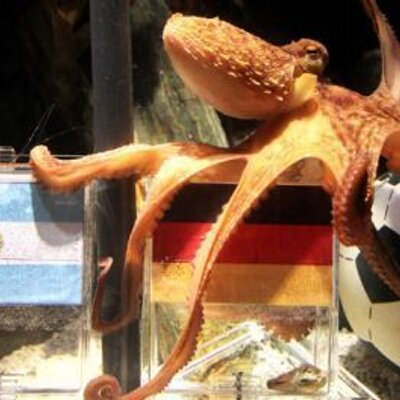
\includegraphics[width=\textwidth, height=\textheight, keepaspectratio=true]{kraken}
}

\frame {
	Underconfidence
}

\frame {
	\begin{itemize}
	\item Not believing your beliefs enough
	\item There is radioactive rain on 8  (instead of 6)
	\item I'm underconfident
	\item People usually aren't underconfident (in forecasting)
	\end{itemize}
}

\frame {
	Overconfidence
}

\frame {
	\begin{itemize}
	\item Believing your beliefs too much
	\item There is radioactive rain on 3 of the next 10 days (instead of 6)
	\item I'm overconfident
	\item Nearly everyone is overconfident
	\end{itemize}
}

\frame {
	You're calibrated if n\% of your n\% forecasts come true.
}

\frame {
	Resolution
}

\frame {
	Willingness to make "daring" predictions (near 0\% or 100\%).
	Predicting always 50\% will be calibrated, but with low resolution.
}

\frame {
	Brier score
}

\frame {
	\begin{itemize}
	\item Score to determine the accuracy of a set of forecasts
	\item 0 is perfect, 0.25 is completely random, 1 is also perfect (but reversed)
	\item Good forecasters achieve scores from ~0.1 to ~0.2
	\end{itemize}
}

\frame {
	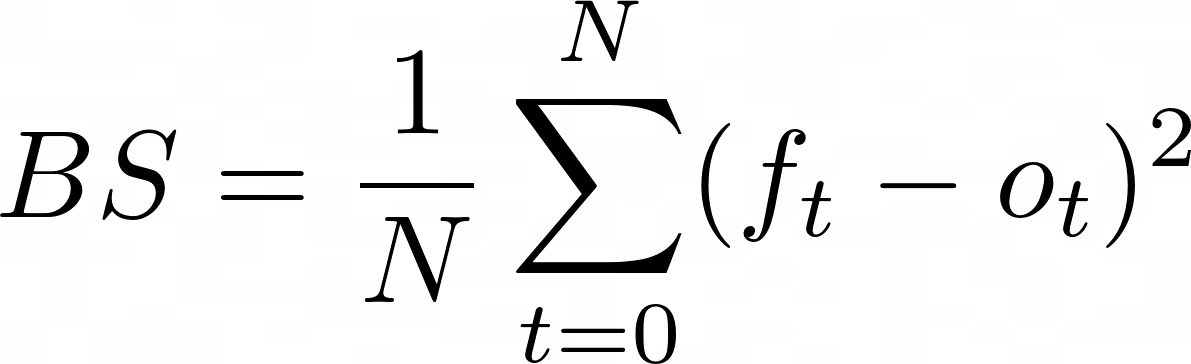
\includegraphics[width=\textwidth, height=\textheight, keepaspectratio=true]{brier}
}

\frame {
	Useful techniques in forecasting
}

\frame {
	Intuition/Practice
}

\frame {
	Yes, your intuition knows a lot about the world, and its forecasting
	abilities can be developed by practice.
}

\frame {
	Just make up some numbers!
}

\frame {
	Base Rates
}

\frame {
	The base rate of an event is the incidence of this kind
	of event happening in the past.
}

\frame {
	Example:
	There was radioactive rain on 20\% of the days in the last year.
	Then 20\% seems like a good first estimate for radioactive rain
	tomorrow.
}

\frame {
	Wisdown of the Crowds/Dialectical Bootstrapping
}

\frame {
	Wisdown of the crowds:
	    Take the estimates of multiple people, use the mean.
	Dialectical bootstrapping:
	    Make multiple different own estimates, use the mean.
}

\frame {
	Extremising
}

\frame {
	When the estimates of different people point in the same direction,
	become more confident.
}

\frame {
	Example:
	7 people independently agree that the probability of radioactive rain
	tomorrow is 65\%. They all have different information, so we can become
	more confident (e.g. 85\%).
}

\frame {
	Extrapolation
}

\frame {
	If something has shown a growth pattern in the past, that
	growth pattern might continue
}

\frame {
	With statistical software, fitting/regression \& extrapolation
	can be done
}

\frame {
	Usually used as a starting point
}

\frame {
	Different kinds of processes
}

\frame {
	Linear
	Constant growth
	Example: Cumulative work done by a single person
}

\frame {
	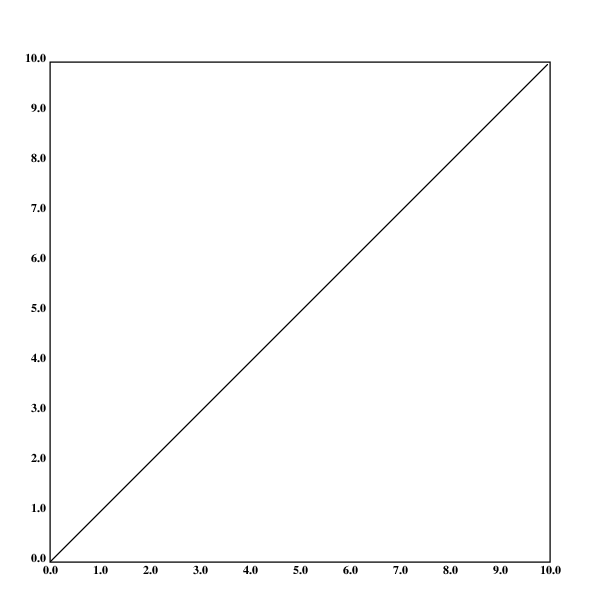
\includegraphics[width=\textwidth, height=\textheight, keepaspectratio=true]{linear}
}

\frame {
	Polynomial (often quadratic)
	Acceleration
	Example: Stopping distance of a car
}

\frame {
	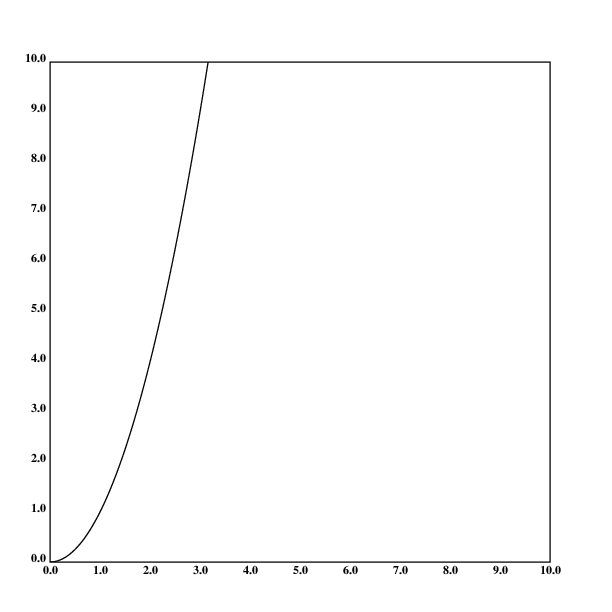
\includegraphics[width=\textwidth, height=\textheight, keepaspectratio=true]{quad}
}

\frame {
	Exponential
	Growth that feeds on itself
	Example: Moore's Law
}

\frame {
	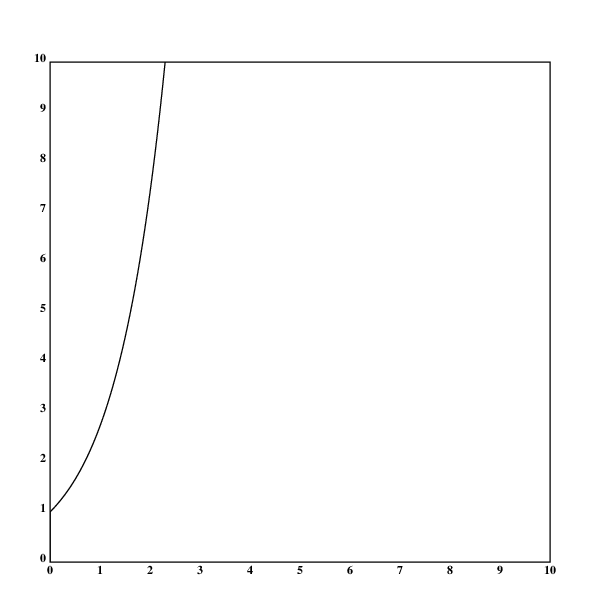
\includegraphics[width=\textwidth, height=\textheight, keepaspectratio=true]{exp}
}

\frame {
	Sigmoid
	Growth that feeds on itself, but is stopped by something
	Example: Spreading of a virus
}

\frame {
	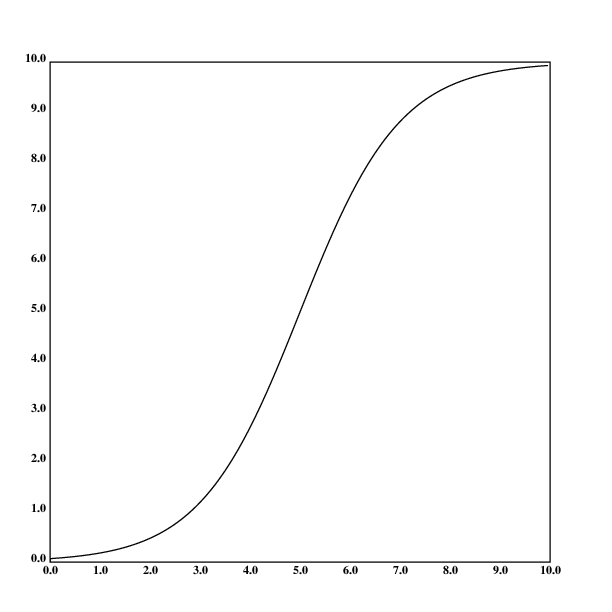
\includegraphics[width=\textwidth, height=\textheight, keepaspectratio=true]{sigmoid}
}

\frame {
	Forecasting Session:
	Make forecasts now, get the results in one month
}

\frame {
	What Is To Be Done?
}

\frame {
	\begin{itemize}
	\item Talk to me about this, I love this stuff
	\item Join an online forecasting tournament/website if you enjoyed this:
		\begin{itemize}
		\item Metaculus (https://www.metaculus.com/questions/) (recommended)
		\item Good Judgement Project (https://www.gjopen.com/)
		\item PredictionBook (https://predictionbook.com/)
		\end{itemize}
	\end{itemize}
	\begin{itemize}
	\item Some Information:
		\begin{itemize}
		\item Ten commandments for Superforecasters (https://fs.blog/2015/12/ten-commandments-for-superforecasters/)
		\end{itemize}
	\end{itemize}
}

\end{document}
